%!TEX root = ../main.tex
%%%%%%%%%%%%%%%%%%%%%%%%%%%%%%%%%%
% Links:
%
% Difficulty:
% Companies: 
%%%%%%%%%%%%%%%%%%%%%%%%%%%%%%%%%%

\chapter{Coin Change Problem}
\label{ch:coin_change}
\section*{Introduction}
The problem discussed in this chapter is considered by many to be a fundamental stepping stone for anyone on the path of mastering Dynamic Programming (see Section \ref{sect:appendix:DP}).
This reputation comes from the fact that this problem encompass all the crucial ingredients of any DP algorithms with the additional benefit of having a statement that is very intuitive as 
it features things like coins and change which are concepts we are all familiar with.

This problem addressed the question of finding the minimum number of coins (of certain given denominations) that add up to a given amount of money. 
Many people, when reading the problem statement of this problem, are tempted to approach it greedily but, as we will see,  this does not always lead us towards the correct answer. 
Moreover, the coin change problem can be seen as an archetype for a whole bunch of DP optimization problems which can be reduced, and solved effortlessly, using the techniques shown in this section (see Chapter \ref{ch:dice_rolls} and \ref{ch:can_jump}, for instance).


\section{Problem statement}
\begin{exercise}
Write a function that given an array of coin denominations $I$ and an integer $t$ representing an amount of money, returns
the minimum number of coins (of any denomination in $I$) that are necessary need to make up that amount. 
You have an infinite amount of coins of each denomination. 
	\begin{example}
		\label{ex:coin_change:example1}
		\hfill \\
		Given $I={1,2,5}$ and $t=11$, the function returns $3$.
		We can change $11$ in many ways, but none of them uses less than $3$ coins:
		\begin{itemize}
			\item two coins of denomination $5$,
			\item and one coin of denomination $1$
		\end{itemize}
	\end{example}

	\begin{example}
		\hfill \\
		Given $I={1,3,4,5}$ and $t=7$, the function returns $2$.
		We can change $7$ by using one coin of value $3$ and one of value $4$.
	\end{example}

	\begin{example}
		\hfill \\
		Given $I={1,5,8}$ and $t=12$, the function returns $4$.
		We can change $12$ by using two coins of value $1$ and two of value $5$.
	\end{example}
\end{exercise}

\section{Clarification Questions}

\begin{QandA}
	\item Is $I$ sorted?
	\begin{answered}
		\textit{No, denomination in $I$ are not sorted.}
	\end{answered}

	\item Can we assume we can always change $t$ using the denomination in $I$?
	\begin{answered}
		\textit{No, and if that is the case the function should return $-1$.}
	\end{answered}
	
\end{QandA}

\section{Discussion}
\label{coin_change:sec:discussion}

\subsubsection{Mathematical definition}
\label{coin_change:sec:mathdefinition}
This problem can be formalized as an optimization problem where the solution is a set of number $X=\{X_0,X_1,\ldots, X_{|I|-1}\}$ of size $|I|$ with each $x_j$ representing how many coins of the denomination $I_j$ are used and the answer is the minimum of 
$
	W(t) = \sum_{j=0}^{|I|-1} X_j
$
subject to:
$
	\sum_{j=0}^{|I|-1} X_j I_j = t
$
where $W(t)$ is total the sum of all the coins used, with a total value of exactly $t$, the target amount.

\subsection{Brute-force}
\label{coin_change:sec:bruteforce}
The brute-force approach is conceptually straightforward and basically consists in checking enumerating every single possible valid combination of coins
and keep track of one with the smallest number of coins in it. A valid combination can be uniquely identified by the array $X$  mentioned above (in Section \ref{coin_change:sec:mathdefinition}).
The enumeration process can be implemented using recursion and backtracking. 
The idea is that we fill $X$ (which initially is filled with zeros) incrementally starting with the first position, $X_0$, which represent the number of coins of the first denomination. 
Every time we try a new value $k$, for $X_0$, we know we are adding $kI_0$ to the overall value of all the coins in $X$, and of course also that we used $k$ coins.
At this point we can continue and try to fill the next position of $X$ knowing have to make up for $t-kI_0$ and that we have used already $k$ coins. We can fill the first position in a similar manner to what we did for the position $0$.
This process can be repeated until either we reach a point where we have nothing to make up for anymore or we still have a certain amount to change but no available denominations.
In the former case we return the number of coins used up to that point, while in the latter we return a value indicating that there is no solution.

An implementation of this idea is shown below in Listing \ref{list:coin_change:bruteforce}.
Notice that the function \inline{change_ways_bruteforce_backtracking_helper} takes $4$ parameters:
\begin{enumerate}
	\item \inline{I}: a purely input parameter containing the denominations,
	\item \inline{t}: the amount we need to make up for,
	\item \inline{j}: the denomination index in $I$ we are currently processing, and
	\item \inline{coin_used}: the number of coin used so far.
\end{enumerate}
The function is initially called with the original value of $j=0$ (because we start with the first denomination), \inline{coin_used = 0} (no coins are used when we start this backtracking process) and \inline{t} is set to be equal to the original amount (the one coming from the main driver function \inline{change_ways_bruteforce}).
As the execution and the recursion unfold $t$ is changed accordingly to the values of the coin used, 
\inline{coin_used} is updated with the number of coin used and $j$ is incremented by one at each recursive call. Figure \ref{fig:coin_change:recursiontree} shows the recursion tree of \inline{change_ways_bruteforce_backtracking_helper} when the input is the one shown in Example \ref{ex:coin_change:example1}; As we can see, there are $4$ ways of changing $4$ by using coin of denominations $\{1,2,3\}$:
\begin{enumerate}
	\item $2+2$ (using two coins of value $2$),
	\item $1+3$, (using one and three coins of values $1$ and $3$, respectively)
	\item $1+1+2$,(using two and one coins of values $1$ and $2$, respectively), and
	\item $1+1+1+1$ (using $4$ coins of value $1$).
\end{enumerate}

\begin{figure}
	\centering
	\label{fig:coin_change:recursiontree}
	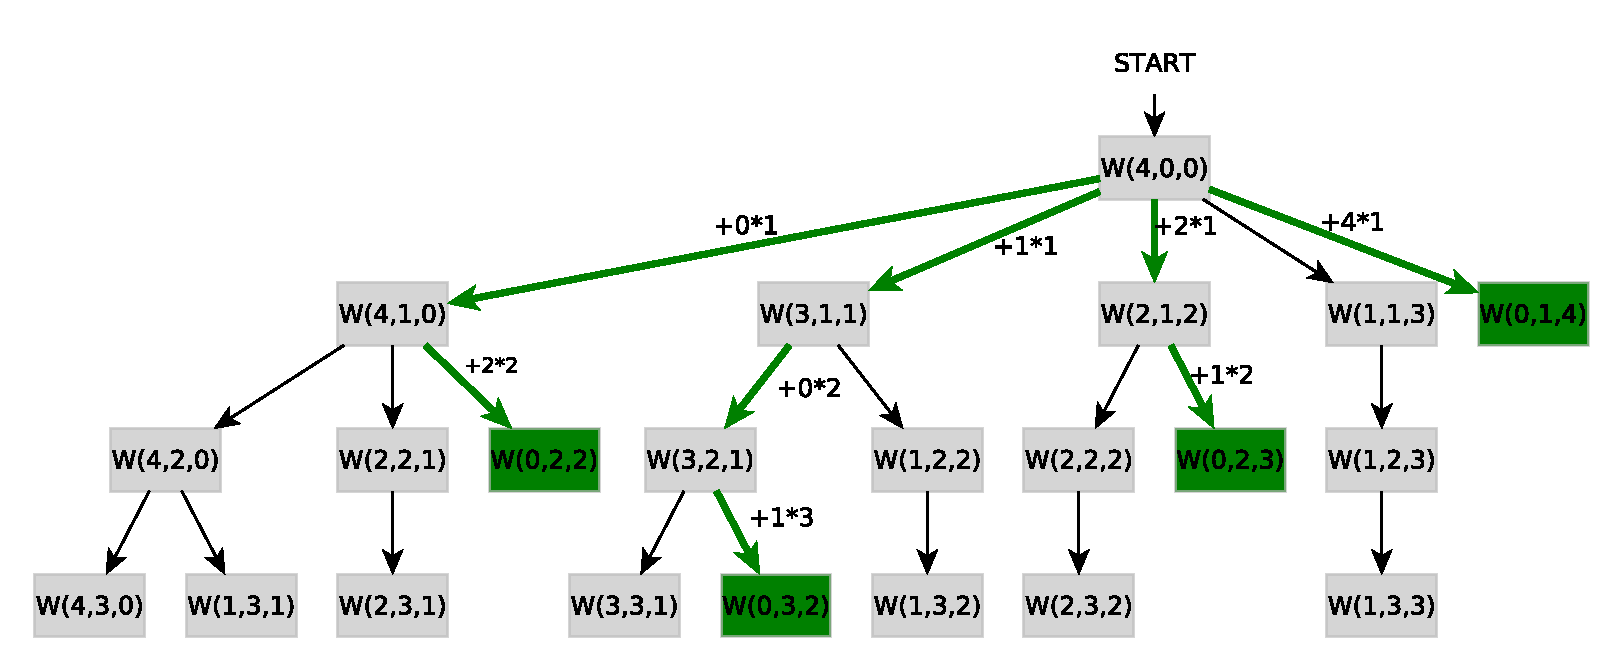
\includegraphics[width=\textwidth]{sources/coin_change/images/recursiontree}
	\captionsetup{singlelinecheck=off}
	\caption{This figure shows the call tree for the recursive function \inline{change_ways_bruteforce_backtracking_helper} on the following input:  $I = \{1,2,3\}$, and $t=4$. Each node contains the only three varying parameters of \inline{change_ways_bruteforce_backtracking_helper} (shortened here as $W$): the first is the current $t$ (the amount that we still need to make up for). The second   is the index to an element of $I$ for the denomination we are considering and the third is the number of coins used so far.
	Moreover, the highlighted paths shows all the valid ways of changing $4$. Note that all the green nodes have the first number equal to zero.}
\end{figure}

\lstinputlisting[language=c++, caption={Backtracking recursive brute-force solution},label=list:coin_change:bruteforce]{sources/coin_change/coin_change_solution3.cpp}

The time complexity of this approach is exponential in $|I|$. As an informal proof consider that for each denomination we at least try either to use zero or one coin. 
Therefore for each element of $I$ we have two choices resulting in $2^{|I|}$ possibilities. 
The space complexity is linear in $|I|$ as in the worst case the depth of the recursive calls do not go lower than $|I|$. This is a direct consequence of the base case, checking for $j >= |I|$.

\subsection{Dynamic Programming - top-down}
\lstinputlisting[language=c++, caption={Sample Caption},label=list:coin_change]{sources/coin_change/coin_change_solution1.cpp}



\section{Common Variations}